\documentclass[a4paper,oneside]{article}
%Compilé avec MacTex
\usepackage[french]{babel}
\usepackage[utf8]{inputenc}
\usepackage[T1]{fontenc}
\usepackage{hyperref} % références dans pdf
\usepackage[tt]{titlepic}
\usepackage{graphicx} % pour images
\usepackage{rotating} % pour rotatebox
\usepackage{lmodern}
\usepackage{amsmath}
\usepackage{amssymb}
\usepackage{mathrsfs}
\usepackage{sistyle}
\usepackage{chngpage}
\usepackage{caption}
\usepackage{epstopdf}
\usepackage{gnuplottex}% pour faire du gnuplot directement dans le latex
\usepackage[nottoc, notlof, notlot]{tocbibind} % pour que bibliographie soit comprise comme un chapitre ou section
\usepackage{appendix} % pour les annexes
\pagestyle{headings} % pour en têtes
\usepackage{mathenv}
  %\usepackage{SIunitx}
%\usepackage{siunitx}%pour les unités SI
\DeclareTextSymbol{\degre}{OT1}{23} %pour le symbole degré
\makeatletter % pour /bigcenter qui permet de s'affranchir des marges pour les images
\newskip\@bigflushglue \@bigflushglue = -100pt plus 1fil

\def\bigcenter{\trivlist \bigcentering\item\relax}
\def\bigcentering{\let\\\@centercr\rightskip\@bigflushglue%
\leftskip\@bigflushglue
\parindent\z@\parfillskip\z@skip}
\def\endbigcenter{\endtrivlist}
\makeatother


\begin{document}

%************************************************************************
%									TITRE
%************************************************************************


\begin{titlepage} % Suppresses headers and footers on the title page

	\centering % Centre everything on the title page

	\scshape % Use small caps for all text on the title page

	\vspace*{\baselineskip} % White space at the top of the page


	\rule{\textwidth}{1.6pt}\vspace*{-\baselineskip}\vspace*{2pt}
	 % Thick horizontal rule
	\rule{\textwidth}{0.4pt} % Thin horizontal rule

	\vspace{0.75\baselineskip} % Whitespace above the title

	{\LARGE Bureau d'\'Etudes :\\
	\vspace{0.75\baselineskip}
	Conception d'un Réacteur Chimique\\
	} % Title

	\vspace{1\baselineskip} % Whitespace below the title
	\rule{\textwidth}{0.4pt}\vspace*{-\baselineskip}\vspace*{3.2pt}
	 % Thin horizontal rule
	\rule{\textwidth}{1.6pt} % Thick horizontal rule
	\vspace{2\baselineskip} % Whitespace after the title block

	%------------------------------------------------
	%	Subtitle
	%------------------------------------------------

	% Subtitle or further description
	Méhodes Numériques : Volumes Finis

	\vspace*{3\baselineskip} % Whitespace under the subtitle

	%------------------------------------------------
	%	Editor(s)
	%------------------------------------------------


	\vspace{0.5\baselineskip} % Whitespace before the editors

	{\scshape\Large Quentin Bergé \\ Adrien Autellet\\} % Editor list

	\vspace{0.5\baselineskip} % Whitespace below the editor list

	\textit{ENSEEIHT} % Editor affiliation

	\vfill % Whitespace between editor names and publisher logo

	%------------------------------------------------
	%	Publisher
	%------------------------------------------------

	
\includegraphics[scale=0.3]{logoN7.png} % changer logo

	\vspace{0.3\baselineskip} % Whitespace under the publisher logo

Juin 2019 % Publication year
\end{titlepage}
\newpage

%Table des Matières
\tableofcontents
\newpage

\section{Introduction}

L'objectif de ce bureau d'études est d'étudier la cinétique chimique lors de l'injection de deux réactifs au sein 
d'un réacteur chimique. Cette cinétique étant fortement influencée par la température, on se propose d'étudier le phénomène 
d'advection-diffusion de cette dernière par la méthode des volumes finis.

\section{Description du Problème}

Selon la configuration schématisée dans la figure ci-dessous, les deux réqctifs sont injectés face-à-face.
Puisque la diffusivité thermique des réactifs est très grande, l'efficacité de l'échangeur est dictée par la cinétique de la réaction qui est très influencée par la température. Cela revient donc à étudier le champ de température sur toute la taille du réacteur mais surtout dans la zone centrale. C'est pour cela que nous analyserons le phénomène d'advection-diffusion de la température par la méthode des volumes finis. 


\begin{figure}[h!]
\bigcenter
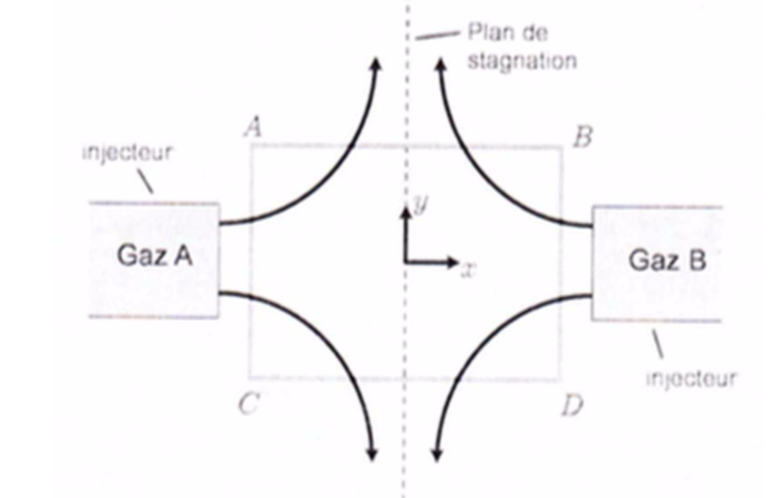
\includegraphics[scale=0.8]{Schema_reacteur.PNG}
\caption{Schéma du système d'injection dans le réacteur chimique}
\end{figure}

Selon le cahier des charges, nous devons respecter certaines scpécifications :
\begin{itemize}
	\item Maillage irregulier en x et y
	\item Schéma amont pour le terme advectif
	\item Schéma centré pour le terme diffusif
	\item Intégration temporelle par la méthode d'Euler explicite
	\item Conditions de Dirchlet avec température gaussienne sur les frontières AC et BD
	\item Conditions de Neumann avec Interpolation des flux diffusifs à partir des flux connus à l'intérieur du domaine
\end{itemize}


\section{Pré-Processeur}
\subsection{Lecture d'un Fichier d'Entrée}

Le fichier d'entrée est disposé dans le dossier RUN et donne accès à certaines variables que l'on peut changer comme des Données Numériques :
\begin{itemize}
	\item temps final
	\item nombre de points en x $N_x$
	\item nombre de points en y $N_y$
\end{itemize}

et comme Données Physiques :
\begin{itemize}
	\item la longueur du domaine \verb?L?
	\item la vitesse carcatéristique des gaz $A$
	\item les coefficients de diffusivité thermiques $\alpha_a$ et $\alpha_b$
\end{itemize}

Ce fichier d'entrée est lu à l'aide de la subroutine \verb?read_data?



\subsection{le Maillage}
Etant donné que nous travaillons avec un code 2D il nous faut mailler le réacteur selon le schéma suivant.
Et puisque la subroutine de transformation de VTS vers Paraview nous fait utiliser des tableaux de taille ($N_x$,$N_y$), nous avons choisit cette structure pour tous nos tableaux.

\begin{figure}[h!]
\bigcenter
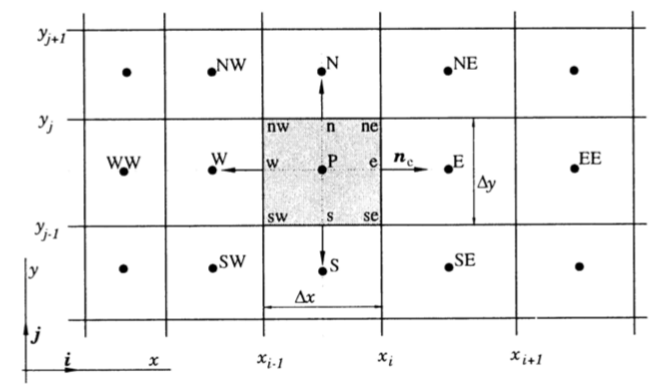
\includegraphics[scale=0.5]{Champ_Vitesse_Maillage/MaillageTheorique.PNG}
\caption{Exemple d'un maillage 2D SOURCE A METTRE Poly Alexei Stoukov}
\end{figure}

Pour ceci nous allons donc utiliser plusieurs tableaux, pour chaque maillage il y aura un tableau pour $x$ et un selon $y$ dépendant de ($i$,$j$) conformément au schéma ci-dessus.

Nous définissons alors 4 maillages différents :
\begin{itemize}
	\item pour les noeuds \verb?xnoeuds? , \verb?ynoeuds?
	\item pour les centres des volumes \verb?xcentre_vol?, \verb?ycentre_col?
	\item pour les faces horizontales \verb?xcentre_faces_horiz?,\verb?ycentre_faces_horiz?
	\item pour les faces verticales \verb?xcentre_faces_vertic?, \verb?ycentre_faces_vertic?
\end{itemize}

On effectue d'abord le maillage sur les noeuds et les centres des volumes, puis on peut composer les faces horizontales et verticales avec ceux-ci.
Tout ces tableaux sont de tailles différentes puisqu'il y a $N_x \times N_y$ noeuds mais ($N_x -1 )\times (N_y -1$) centres.
C'est pourquoi il faudra faire attention à la taille des tableaux quand on les allouera.
Ces tableaux sont en allocations dynamiques, on alloue uniquement la mémoire qui sera nécéssaire aux tableaux afin de ne pas trop en consommer en accord avec les données du fichier d'entrée. 


Etant donné qu'on lit sur le fichier d'entrée $N_x$,$N_y$, on va calculer les pas \verb?dx? et \verb?dy? 
\[
 d_{x,y} = \frac{L}{N_{x,y} -1}
\]

De cette façon on a pu obtenir un maillage régulier visualisé comme ceci avec ParaView.

\begin{figure}[h!]
\bigcenter
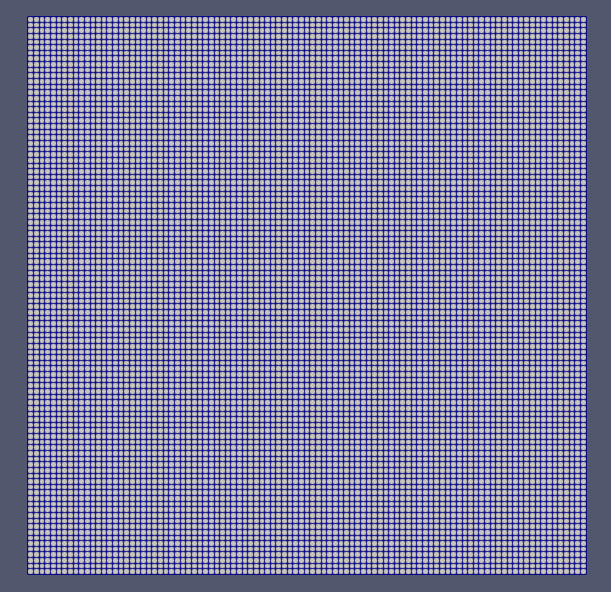
\includegraphics[scale=0.4]{Champ_Vitesse_Maillage/maillage100100.PNG}
\caption{Maillage (100,100) visualisé sur Paraview}
\end{figure}

Ce maillage est réalisé à l'aide de la subroutine \verb?maillage?

\subsection{Champ des Vitesses}

On a ensuite pu calculer le champ des vitesses aux centres des volumes selon 

\begin{equation*}
\begin{cases}
 u = A \cos \left( \pi \left( {\frac{x}{L} - \frac{1}{2}} \right) \right)  \sin \left( \pi \left( \frac{y}{L} - \frac{1}{2}\right) \right) \\
 v = -A \sin \left( \pi \left( {\frac{x}{L} - \frac{1}{2}} \right) \right)  \cos \left( \pi \left( \frac{y}{L} - \frac{1}{2}\right) \right) \\
\end{cases}
\end{equation*}

avec $A$ paramètre caractéristique de la vitesse maximale du gaz, ici choisi à 0,05 $m/s$.\\
Voici ce qu'on obtient en le modélisant sur ParaView, on observe bien la symétrie des 2 profils de vitesse.

\begin{figure}[h!]
\centering
        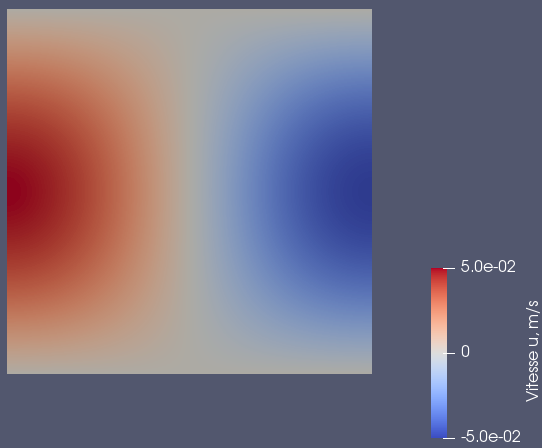
\includegraphics[scale=0.4]{Champ_Vitesse_Maillage/Champ_Vitesse_u.png}
        \caption{Champ des vitesses sur $u$ pour un maillage (100,100)}

\end{figure}

\begin{figure}[h!]
	\centering
        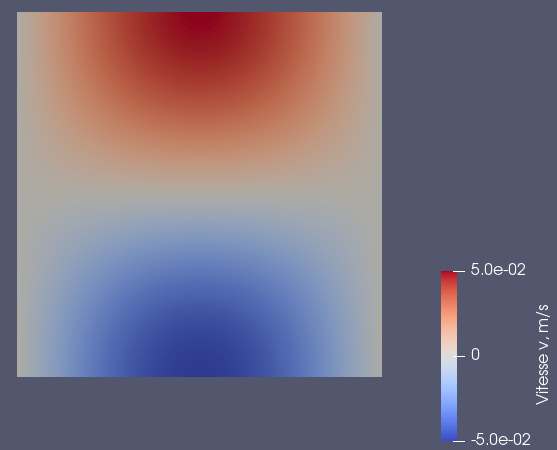
\includegraphics[scale=0.4]{Champ_Vitesse_Maillage/Champ_Vitesse_v.png}
        \caption{Champ des vitesses sur $v$ pour un maillage (100,100)}
\end{figure}

Ce calcul du champ des vitesses est réalisé à l'aide de la subroutine \verb?champ_vitesse?

\subsection{Calcul du Pas de Temps}

\subsection{Para View}

Para View est un logiciel libre de visualisation de données. 
Il nous permet à l'aide de la subroutine fournie \verb?VTSWriter? en fournissant certains arguments d'afficher nos résultats dans ce format.

\section{Discrétisation}

\subsection{Architecture}
???





\section{Validation}


\section{Exploitation}


\section{Conclusion}



\end{document}
